\section{Approach}
\newcommand{\ROY}[1]{\textcolor{blue}{Roy: #1}}


The multi-turn response selection tasks represent each dialogue as a triple $T=\langle C, R, L\rangle$, where $C=\{t_1, t_2,...,t_n\}$ represents the history turns. $R$ is a candidate response and $L$ is the $0/1$ label indicating whether the $R$ is the correct response or a negative candidate. To incorporate the dependency information between the history turns, we design a straight-forward algorithm to extract the dialogue history $C$ into dialogues threads $\langle C_1, C_2, ..., C_M\rangle$ based on the predicted dependencies, along with an elaborately designed model to find the function $F(C_1, C_2, ..., C_M, R)$, which measures the matching score of each $(C, R)$ pair. Both extraction algorithm and the model will be explained in this section.

\subsection{Dialogue Extraction Algorithm}
\label{sec:DSA}
Since it's impossible for the large pretrained language models to take all of the dialogue history turns as the input under the computational power nowadays, these models usually set a truncate window and just consider the top-k most recent turns or tokens. However, several dialogue threads may exist concurrently in two-party~\cite{DuPX17} or multi-party dialogues~\cite{TanWGWPGCY19}. Such coarse-grained truncating operation may not only bring in redundant turns from 
other dialogue threads, but also exclude the expected turns given earlier 
in current dialogue thread, hurting the representation capability of 
the pretrained language model.

\begin{figure}
	\centering
	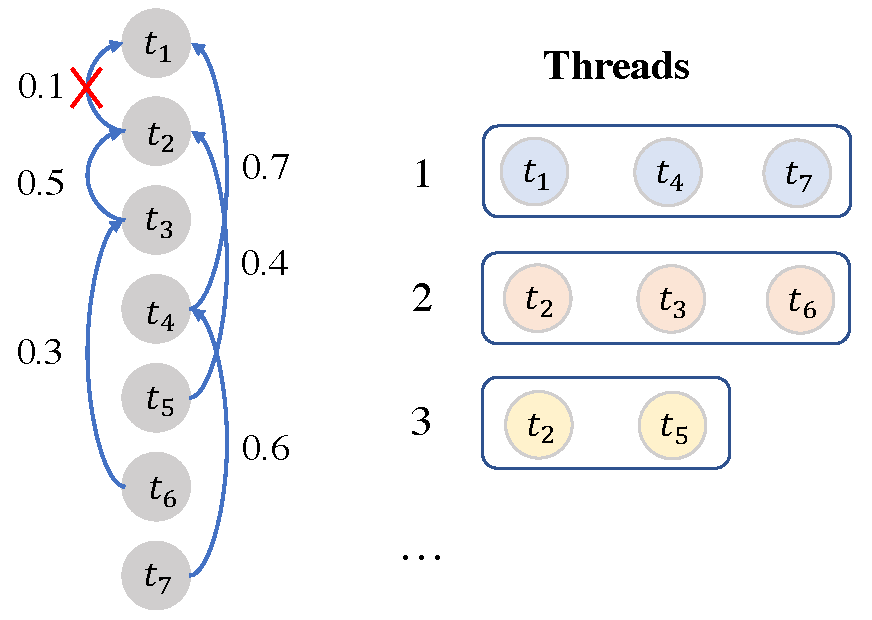
\includegraphics[scale=0.42]{pic/algorithm.pdf}
	\caption{An example of the algorithm when $P=0.2$}
	\label{fig:algorithm}
\end{figure}


Motivated by the above, we utilize the discourse dependency parsing model for dialogues proposed by Shi and Huang~\shortcite{ShiH19}. It is a deep sequential model which achieves the state-of-the-art performance on the STAC corpus based on SDRT discourse theory. Here, we avoid the complex SDRT theory with 16 relations types between EDUs, and only consider the dependency relation ``reply-to'' between the turns in a dialogue history. 
The model scans through a dialogue and predict the most likely parent turns for each turn. 
It finally constructs a dependency tree for a dialogue history with confidence score 
on each edge.

%\IncMargin{1em} 
\begin{algorithm}
	\scriptsize
	\SetAlgoNoLine 
	\SetKwInOut{Input}{\textbf{Input}}
	\SetKwInOut{Output}{\textbf{Output}} 
	
	\Input
	{
		The dependency tree $T$ with confidence score on each edge $e_{ji}=(t_i, t_j, P_{ji})$, where $i.j=1, 2, ..., n$ and $j>i$;\\
		The threshold for the confidence score $P$.
	}
	\Output{
		The threads $C'=\langle C_1, C_2, ..., C_M\rangle$, and each is made up a sequence of turns.
	}
	\BlankLine
	
	\For {$e_{ji}$ in $T$}{
		\If{$P_{ji}<P$}{delete $e_{ji}$ from $T$}
	}
	The forest $T' = T$\\
	The set of threads $C'=\emptyset$\\
	\For{each leaf node in $T'$ }{
		$C_{tmp} =$ all the node from the leaf node to the corresponding root.\\
		$C'=C'\cup C_{tmp}$
	}
	Rank the threads in $C'$ based on the index of the leaf node in descending order.
	
	\caption{The Dialogue Extraction Algorithm\label{alg:A}}
	\label{alg:DSA}
\end{algorithm}
%\DecMargin{1em}


The dialogue extraction algorithm is designed to extract original long history into the dialogue threads according to dependency tree $T$ and confidence scores. The algorithm is 
depicted in \algoref{alg:A}. $e_{ji}$ is a directed edge with head $t_i$ and tail $t_j$, 
indicating that turn $j$ is a reply of turn $i$ with probability $P_{ji}$.
The threshold $P$ is a hyper-parameter. It is noteworthy that we still follow the intuition 
that the turns closer to the responses are more informative than others. 
The threads are returned in ascending order according to the distance between 
the last turns in each thread and the response. 
An illustration of the algorithm is shown in Figure \ref{fig:algorithm}.


\subsection{Thread-based Encoder Model}
\label{sec:tem}
In the work from Humeau et al.~\shortcite{humeau2019poly}, they use a pretrained language model as the context encoder and generate the embedding for dialogue history. Inspired by this work, we also utilize the pretrained language model to encode the natural texts into meaningful representations.

Given threads $\langle C_1, C_2, ..., C_M \rangle$, each thead is regarded as a self-contained dialogue thread. We want to utilize a pretrained language model to encode the content of each dialogue thread and another pretrained language model to encode the candidate respectively. 
If the candidate representation matches well with one or more thread representations, 
that candidate is probably the correct response. 

The architecture of our model (shown in \figref{fig:model1}) can be divided into two layers: Encoder Layer and Matching Layer.

\subsubsection{Encoder Layer}
We use the pretrained language model released by Humeau et al.~\shortcite{humeau2019poly}. This large pretrained Tranformer model has the same architecture as BERT-base \cite{DevlinCLT19}. It has 12 layers, 12 attention heads and 768 hidden size. Different from the original one trained on BooksCorpus and Wikipedia, the new language model is instead trained on Reddit~\cite{abs-1904-06472}, a large dialogue dataset with around 727M context-response pairs. The pretraining tasks include masked language model and next utterance prediction~\footnote{``Utterance'' and ``turn'' are 
interchangeable in this paper.}. Finally, the pretrained model can be used for 
a wide range of multi-sentence selection tasks with fine-tuning.

The encoder layer uses two Transformers, $T_1(\cdot)$ and $T_2(\cdot)$, both initialized with the pretrained weights. $T_1(\cdot)$ is used for encoding threads, and all of the turns in a thread is concatenated into a long sequence in chronological order as the input. 
$T_2(\cdot)$ is used for encoding the candidate. The inputs to the 
Transformer encoder are surrounded by the special token $[S]$, 
consistent with the operations during pre-training.

Above the Transformer encoder is an aggregation layer $agr(\cdot)$ that aggregates
a sequence of vectors produced by the encoder into one vector. 
Here we use the averaged vector as the final representation for an encoder block. 
Finally, the threads and response can be encoded as follows:

\begin{equation}
\begin{aligned}
C^{emb}_m&=agr(T_1(C_m))\\
R^{emb}&=agr(T_2(R)),
\end{aligned}
\end{equation}
where $m=1,2,...M$.

%We get $<C^{emb}_1, C^{emb}_2, ...>$ and $R^{emb}$


\begin{figure}
	\centering
	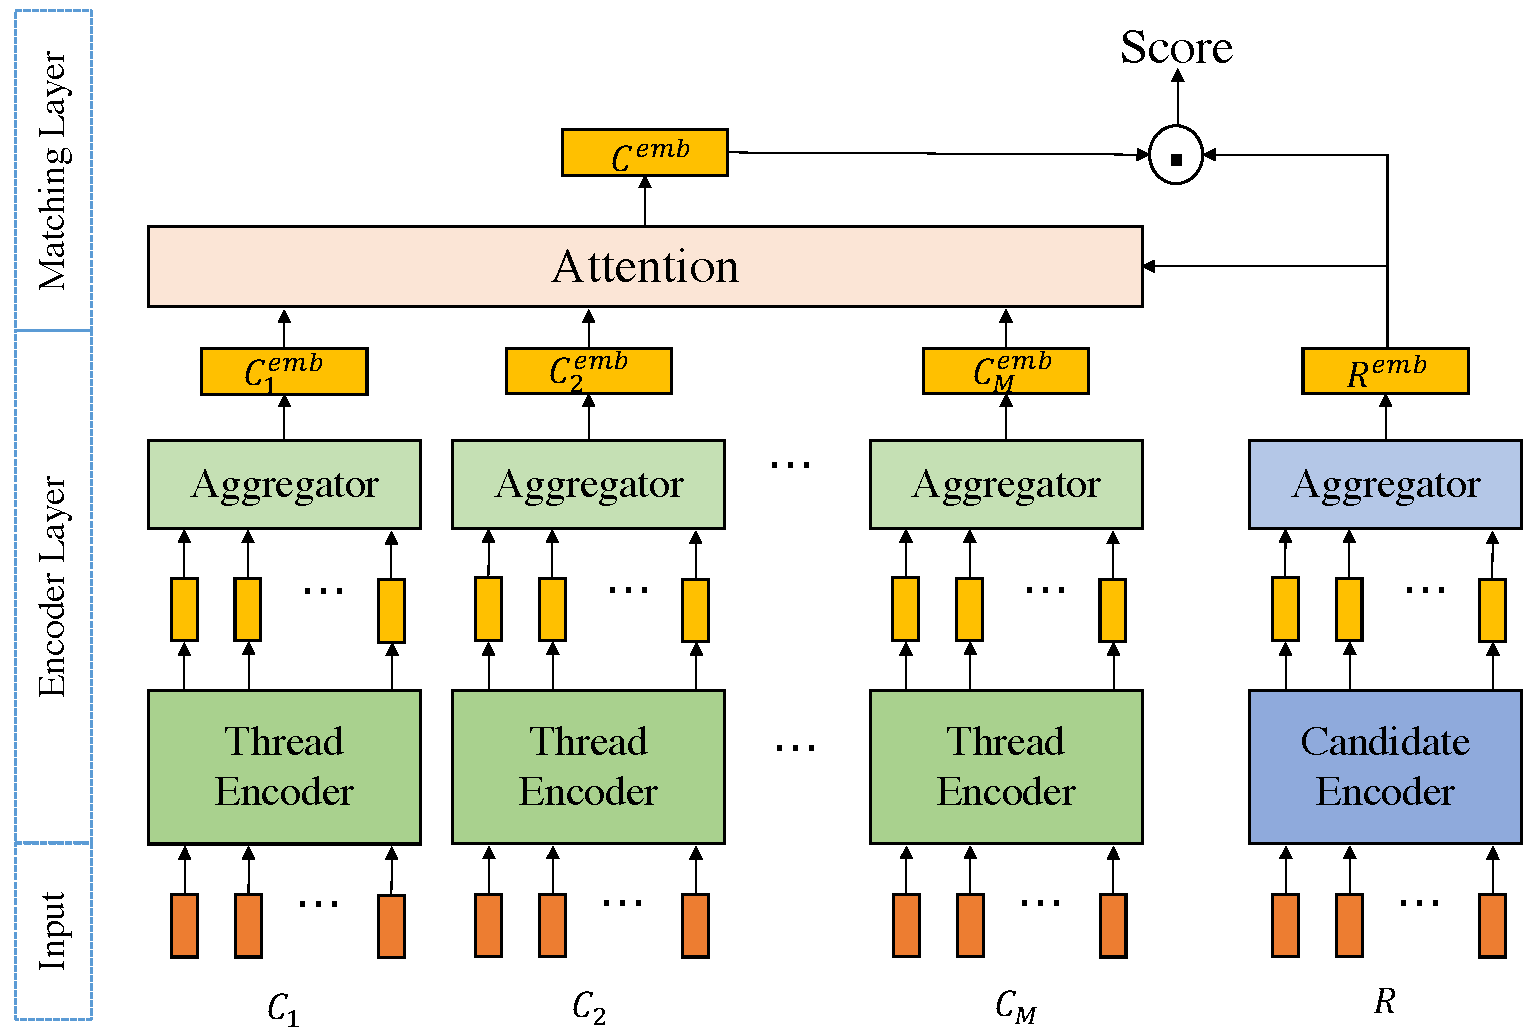
\includegraphics[scale=0.32]{pic/model.pdf}
	\caption{The architecture of Thread-Encoder model. All of the blocks in the same color share parameters.}
	\label{fig:model1}
\end{figure}

\subsubsection{Matching Layer}

Given the encoded threads $\langle C^{emb}_1, C^{emb}_2, ..., C^{emb}_M\rangle$ and candidate $R^{emb}$, we further use an attention layer to distill the information from the threads by attending the query $R^{emb}$ to each $C_m^{emb}$:

\begin{equation}
\begin{aligned}
C^{emb}&=\sum_{m=1}^Mw_mC^{emb}_m
\end{aligned}
\end{equation}
where

\begin{equation}
\begin{aligned}
s_m &= (R^{emb})^\top \cdot C^{emb}_m\\
w_m &= \exp(s_m)/\sum_{k=1}^M\exp(s_k)
\end{aligned}
\end{equation}

The final matching score is given by:
\begin{equation}
\begin{aligned}
S = F(C_1, C_2, ..., C_M, R) = (R^{emb})^\top\cdot C^{emb}
\end{aligned}
\label{eq:matching_score}
\end{equation}

We consider the other correct responses in a mini-batch as the negative candidates to accelerate the training process~\cite{MazareHRB18}. The whole model is trained to minimize the cross-entropy loss as follows:
\begin{equation}
\begin{aligned}
loss = - \frac{1}{A}\sum_{a=1}^{A}\sum_{b=1}^{A} L_{ab}\log(S_{ab})
\end{aligned}
\end{equation}
where $A$ is the batch size. $L_{ab}$ equals $1$ when $a=b$, otherwise $0$. $S_{ab}$ is the matching score in \eqnref{eq:matching_score}.

